\PassOptionsToPackage{unicode=true}{hyperref} % options for packages loaded elsewhere
\PassOptionsToPackage{hyphens}{url}
%
\documentclass[english,]{article}
\usepackage{lmodern}
\usepackage{amssymb,amsmath}
\usepackage{ifxetex,ifluatex}
\usepackage{fixltx2e} % provides \textsubscript
\ifnum 0\ifxetex 1\fi\ifluatex 1\fi=0 % if pdftex
  \usepackage[T1]{fontenc}
  \usepackage[utf8]{inputenc}
  \usepackage{textcomp} % provides euro and other symbols
\else % if luatex or xelatex
  \usepackage{unicode-math}
  \defaultfontfeatures{Ligatures=TeX,Scale=MatchLowercase}
\fi
% use upquote if available, for straight quotes in verbatim environments
\IfFileExists{upquote.sty}{\usepackage{upquote}}{}
% use microtype if available
\IfFileExists{microtype.sty}{%
\usepackage[]{microtype}
\UseMicrotypeSet[protrusion]{basicmath} % disable protrusion for tt fonts
}{}
\IfFileExists{parskip.sty}{%
\usepackage{parskip}
}{% else
\setlength{\parindent}{0pt}
\setlength{\parskip}{6pt plus 2pt minus 1pt}
}
\usepackage{hyperref}
\hypersetup{
            pdftitle={My Resume},
            pdfborder={0 0 0},
            breaklinks=true}
\urlstyle{same}  % don't use monospace font for urls
\usepackage{graphicx,grffile}
\makeatletter
\def\maxwidth{\ifdim\Gin@nat@width>\linewidth\linewidth\else\Gin@nat@width\fi}
\def\maxheight{\ifdim\Gin@nat@height>\textheight\textheight\else\Gin@nat@height\fi}
\makeatother
% Scale images if necessary, so that they will not overflow the page
% margins by default, and it is still possible to overwrite the defaults
% using explicit options in \includegraphics[width, height, ...]{}
\setkeys{Gin}{width=\maxwidth,height=\maxheight,keepaspectratio}
\setlength{\emergencystretch}{3em}  % prevent overfull lines
\providecommand{\tightlist}{%
  \setlength{\itemsep}{0pt}\setlength{\parskip}{0pt}}
\setcounter{secnumdepth}{0}
% Redefines (sub)paragraphs to behave more like sections
\ifx\paragraph\undefined\else
\let\oldparagraph\paragraph
\renewcommand{\paragraph}[1]{\oldparagraph{#1}\mbox{}}
\fi
\ifx\subparagraph\undefined\else
\let\oldsubparagraph\subparagraph
\renewcommand{\subparagraph}[1]{\oldsubparagraph{#1}\mbox{}}
\fi

% set default figure placement to htbp
\makeatletter
\def\fps@figure{htbp}
\makeatother

\ifnum 0\ifxetex 1\fi\ifluatex 1\fi=0 % if pdftex
  \usepackage[shorthands=off,main=english]{babel}
\else
  % load polyglossia as late as possible as it *could* call bidi if RTL lang (e.g. Hebrew or Arabic)
  \usepackage{polyglossia}
  \setmainlanguage[]{english}
\fi

\title{My Resume}
\date{}

\begin{document}
\maketitle

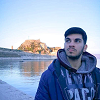
\includegraphics{/online-cv/assets/images/profile.png}

\hypertarget{polycarpos-andreou}{%
\section{Polycarpos Andreou}\label{polycarpos-andreou}}

\begin{itemize}
\tightlist
\item
  \emph{} \href{mailto:p17andr2@ionio.gr}{\nolinkurl{p17andr2@ionio.gr}}
\item
  \emph{} \href{http://github.com/polycarpos}{polycarpos}
\end{itemize}

\hypertarget{education}{%
\subsection{Education}\label{education}}

\hypertarget{section}{%
\paragraph{}\label{section}}

\hypertarget{university-of-ionio}{%
\subparagraph{University of Ionio}\label{university-of-ionio}}

2018 - 20

\hypertarget{section-1}{%
\paragraph{}\label{section-1}}

\hypertarget{ionio-university}{%
\subparagraph{Ionio University}\label{ionio-university}}

2018 - 20

\hypertarget{languages}{%
\subsection{Languages}\label{languages}}

\begin{itemize}
\tightlist
\item
  English {(Native)}
\item
  {()}
\item
  {()}
\end{itemize}

\hypertarget{interests}{%
\subsection{Interests}\label{interests}}

\begin{itemize}
\item
  Gaming
\item
\item
\end{itemize}

\hypertarget{about-theme}{%
\subsection{About Theme}\label{about-theme}}

\begin{itemize}
\tightlist
\item
  \href{https://www.youtube.com/watch?v=Jnmj1dXDbNk}{How to use?}
\item
  \href{https://github.com/sharu725/online-cv}{Star}
\end{itemize}

\hypertarget{career-profile}{%
\subsection{\texorpdfstring{{ \emph{} \emph{} } Career
Profile}{    Career Profile}}\label{career-profile}}

My name is Polycarpos Andreou and I am an undergraduate student at
Ionian University, Department of Informatics, based at Corfu. I was born
in the town of Nicosia,Cyprus,at 5/6/1999

\hypertarget{experiences}{%
\subsection{\texorpdfstring{{ \emph{} \emph{} }
Experiences}{    Experiences}}\label{experiences}}

\hypertarget{section-2}{%
\subsubsection{}\label{section-2}}

2018 -

\begin{itemize}
\tightlist
\item
  Bullet point
\item
  Bullet point
\end{itemize}

\hypertarget{senior-software-engineer}{%
\subsubsection{Senior Software
Engineer}\label{senior-software-engineer}}

2018 - 20

\begin{itemize}
\tightlist
\item
  Bullet point
\item
  Bullet point
\end{itemize}

\hypertarget{section-3}{%
\subsubsection{}\label{section-3}}

2018 - 20

\begin{itemize}
\tightlist
\item
  Bullet point
\item
  Bullet point
\end{itemize}

\hypertarget{projects}{%
\subsection{\texorpdfstring{{ \emph{} \emph{} }
Projects}{    Projects}}\label{projects}}

{ }

{ }

{ }

{ }

{ }

\hypertarget{publications}{%
\subsection{\texorpdfstring{{ \emph{} \emph{} }
Publications}{    Publications}}\label{publications}}

You can list your publications in this section. Lorem ipsum dolor sit
amet, consectetur adipiscing elit. Vestibulum et ligula in nunc bibendum
fringilla a eu lectus.

\hypertarget{section-4}{%
\subsection{\texorpdfstring{{ \emph{} \emph{} }}{   }}\label{section-4}}

\hypertarget{python}{%
\subsubsection{Python}\label{python}}

\hypertarget{javascript}{%
\subsubsection{Javascript}\label{javascript}}

\hypertarget{c}{%
\subsubsection{C++}\label{c}}

\hypertarget{c-1}{%
\subsubsection{C}\label{c-1}}

\hypertarget{section-5}{%
\subsubsection{}\label{section-5}}

\hypertarget{section-6}{%
\subsubsection{}\label{section-6}}

{Designed with \emph{} by \href{http://themes.3rdwavemedia.com}{Xiaoying
Riley}}

\end{document}
